\part{title}%\chapter*{Introducción}\label{chapter:introduction}
\begin{introduction}
	Desde tiempos de antaño el hombre se ha visto en la necesidad imperiosa de manejar de la manera más adecuada posible sus recursos, no solo para conseguir prolongar la vida de estos, sino además para contar con una aceptada utilización de los mismos. Uno de los principales problemas que aqueja a la sociedad actual es la dificultad que se presenta para garantizar un óptimo manejo de nuestro \textit{tiempo}.
	
	La denominada \textit{gestión del tiempo} hace referencia a la forma en que cada uno organiza y planifica cuánto invierte en actividades específicas; pasar más horas en la empresa no significa ser más eficiente o productivo; por ello, es fundamental una adecuada gestión del horario en el trabajo, lo que permitiría lograr más con menos esfuerzo. Cuando se aprende a administrar mejor el día a día y las labores cotidianas se mejora la capacidad de concentración, lo que trae consigo un mayor enfoque y por tanto una mayor eficiencia. Gestionar el tiempo nos permite realizar las tareas con más rapidez y que la jornada laboral sea más efectiva y se aproveche mejor.
	
	En muchos escenarios cotidianos la planificación de las actividades se realiza solamente de manera irreal, por otro lado, existen ámbitos donde se hace necesario garantizar una manipulación detallada de todo el proceso.
	
	Con la llegada de las tecnologías actuales y la facilidad con que las personas cambian de actividad, el desarrollo de un software que garantice una planificación de nuestra agenda diaria, resulta casi imprescindible.
	
	Un ejemplo claro donde sin duda se comprueba el proceso antes expuesto, es la gestión de las actividades de un centro de estudios y más aún en esta época donde contamos con grandes instituciones universitarias que albergan a cientos de estudiantes con diferentes planes de trabajo y manejan una gran cantidad de recursos y útiles.
	
	Quizá muchos consideren que realizar la labor de confección de un horario para una institución universitaria es algo sencillo, pero cabe destacar que la persona encargada de dicha labor, emplea un valioso tiempo en esto; puesto que hay que preveer que no existan colisiones entre los turnos, los locales, los profesores, además de garantizar que todas las actividades se realicen con la frecuencia que corresponde para garantizar el aceptado desarrollo del proceso de aprendizaje por parte del estudiantado.
	
	Resulta llamativo como un gran número de universidades cubanas hoy en día aún no cuentan con un sistema propio (o de terceros) para realizar las tareas de confección del horario; sino que en la mayoría de los casos usan softwares como \textit{Microsoft Excel} para gestionar el mismo; lo cual, sin lugar a dudas es sumamente ineficiente y genera un esfuerzo extra para la persona que está desarrollando el mismo, quién sin lugar a dudas debe tener otra serie de tareas que requieran de más importancia.
	
	El trabajo en cuestión persigue presentar un software para proporcionar un sistema que permita manejar el sistema de turnos de clases de la \textit{Facultad de Matemática y Computación} de \textit{La Universidad de La Habana}.
	
	\section{Motivación}
	Desde hace poco más de 10 años en la Facultad de Matemática y Computación se ha venido gestado la idea de presentar un modelo de horario propio que sea capaz de satisfacer las necesidades internas de la misma. Con anterioridad se han realizado otras tesis de diplomas dedicadas a abordar cuestiones más especifícas relacionadas con esta índole; dígase: manejo de restricciones, generación automática de horarios, entre otros aspectos. 
	
	Las herramientas analizadas previamente, que resolvían el problema del horario, en su mayoría presentaban carencias que se consideraron escenciales a la hora de darle solución al asunto que estamos abordando. Dichas carencias se manejaron dentro del software presentado para garantizar que fueran cubiertas y erradicadas en su totalidad.
	
	Los beneficios finales que ofrecerá el software llaman la atención y es sumamente viable tratarlos como aspectos motivadores a la hora de analizar el resultado final. Se contará por ejemplo, con un sistema de restricciones asociado a todas las entidades del sistema y no solo centrado en los turnos de clases y los profesores; aunque es válido notar que casi todas las condiciones impuestas se relacionan con estos campos. 
	
	El software posibilitará también contar con un sistema centralizado, alojado dentro del nodo de la facultad, lo que hará posible que se pueda acceder en tiempo real por todos los estudiantes y los profesores. Además esto hará más factible la distribución y la organización interna de la institución, puesto que cualquier cambio dentro del sistema, puede ser analizado inmediatamente por todos los interesados.
	
	La edición y el mantenimiento del software, también se realizará de manera relativamente sencilla, con esto se garantiza que se pueda adicionar en el futuro cualquier otra funcionalidad que se considere necesaria o que aporte algún beneficio a la universidad. 
	
	Los profesores son considerados usuarios privilegiados dentro de la aplicación, pues se permite que estos interactuen directamente con los turnos y que muestren sin necesidad de ser administradores, sus inconformidades - por medio de las restricciones -  con la distribución presentada.
	
	Para la persona encargada de la creación del horario, un sistema dedicado especialmente a esto, trae consigo una mejora sustancial; pues es posible detectar datos erróneos durante la confección, se puede tener un control detallado de los profesores, así como de la gestión de locales para poder determinar fácilmente cuáles se encuentran disponibles en un momento y espacio determinado.
	
	En muchos casos es necesario obtener aulas vacías, simplemente para dedicarlas a otras actividad o porque se pretenden usar en otro tipo de eventos. En un gran número de casos esto puede traer un trabajo extra para la persona encargada de realizar tal gestión. El sistema propuesto posibilita que dicha tarea se realice en cuestiones de segundos y sin esfuerzo alguno, debido a que se proporcionan varias vistas o formas de representar el conjunto de turnos que ofrecen una solucióna al problema que se plantea. La distribución por recursos, cubre tal aspecto; pues es posible indentificar todos los locales dentro de la facultad y los horarios en que están ocupados o libres los mismos; además empleando los filtros personalizados se puede hacer incluso más sencilla la tarea.

	
	\section{Objetivos}
	Se tiene como \textbf{objetivo general} presentar una aplicación web que cubra las carencias y dificultades que se exhiben en la facultad de Matemática y Computación de La Universidad de La Habana con respecto a la gestión, distribución y creación del sistema de horarios. 
	La aplicación debe ser lo más sencilla posible para permitir que todo tipo de usuarios interactúen con ella. Como \textbf{objetivos más específicos}, el sistema deberá:
	\begin{enumerate}
		\item Identificar las colisiones presentes entre los turnos, profesores y locales.
		\item Mostrar diversas vistas que hagan posible el chequeo de los turnos de la manera más productiva posible (vista de locales, diaria, por semanas, mensual).
		\item Visualizar en culquier momento que se considere necesario, no solo el horario completo sino secciones específicas del mismo.
		\item Permitir la generación de archivos en formato \textit{Excel}, para ser exportados, y que cuenten con toda la distribución de los turnos de clase.
		\item Permitir el manejo de restricciones o condiciones impuestas sobre todas las entidades del sistema y refelejar el cumplimiento (o no) de estas en una sección dedicada.
		\item Ofrecer un manejo de los profesores, asignaturas, grupos, locales y demás aspectos relacionados con una institución educacional.
		\item Cubrir el manejo de varias facultades a la vez e incluso, llegado a ser el caso de varias universidades. 
	\end{enumerate}
	
	El presente trabajo se estructura como se detalla a continuación: en el capítulo 1 se mostrará todo lo referente al estado del arte, así como una descripción de los softwares y herramientas previamente analizados, mostrando además la carencia de estos y por consiguiente la necesidad de construir uno propio que cubra las necesidades internas de la facultad. En el capítulo 2 se presenta una descripción más detallada del problema así como el enfoque de solución ofrecido. Por último en el capítulo 3 se describirán todos los detalles de implementación referentes al software presentado.
	
	\section{Convenciones de estilos}
	
	Para el presente documento, se mostrarán una serie de figuras o diagramas, para facilitar la comprensión del lector. A continuación se presenta una descripción de las convensiones seguidas para construir las mismas.
	
	\begin{figure}[h!]
		\centering
		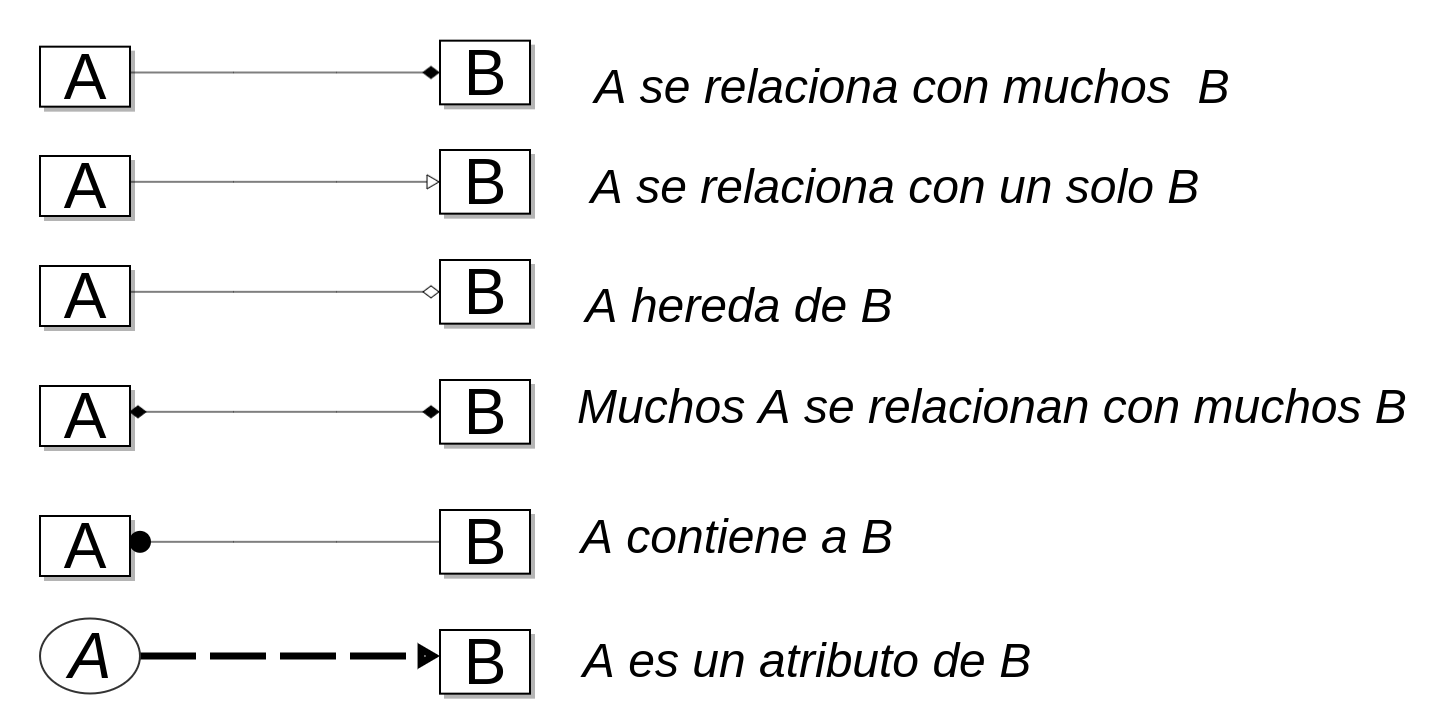
\includegraphics[width=1\linewidth]{images/Introduction/style_conventions}
		\caption{Convenciones de estilos}
		\label{fig:style_conventions}
	\end{figure}
	
	

\end{introduction}
